% fig_pipeline.tex -- code pipeline of the consolidated replication package (pipeline/run.sh stages 00-09).
% Updated 2026-11-05 to the consolidated layout on branch consolidate-p1 (58-file manifest). Script names match the manifest.
% If the stage-01 merge (build_panel.py) is committed, replace the stage-01 script names with build_panel.py <step>.
% Requires tikz (already loaded in main.tex). Usage: % fig_pipeline.tex -- code pipeline of the consolidated replication package (pipeline/run.sh stages 00-09).
% Updated 2026-11-05 to the consolidated layout on branch consolidate-p1 (58-file manifest). Script names match the manifest.
% If the stage-01 merge (build_panel.py) is committed, replace the stage-01 script names with build_panel.py <step>.
% Requires tikz (already loaded in main.tex). Usage: % fig_pipeline.tex -- code pipeline of the consolidated replication package (pipeline/run.sh stages 00-09).
% Updated 2026-11-05 to the consolidated layout on branch consolidate-p1 (58-file manifest). Script names match the manifest.
% If the stage-01 merge (build_panel.py) is committed, replace the stage-01 script names with build_panel.py <step>.
% Requires tikz (already loaded in main.tex). Usage: % fig_pipeline.tex -- code pipeline of the consolidated replication package (pipeline/run.sh stages 00-09).
% Updated 2026-11-05 to the consolidated layout on branch consolidate-p1 (58-file manifest). Script names match the manifest.
% If the stage-01 merge (build_panel.py) is committed, replace the stage-01 script names with build_panel.py <step>.
% Requires tikz (already loaded in main.tex). Usage: \input{figures/fig_pipeline.tex}
\usetikzlibrary{positioning, arrows.meta, calc}
\begin{figure}[!htbp]
\centering
\resizebox{\textwidth}{!}{%
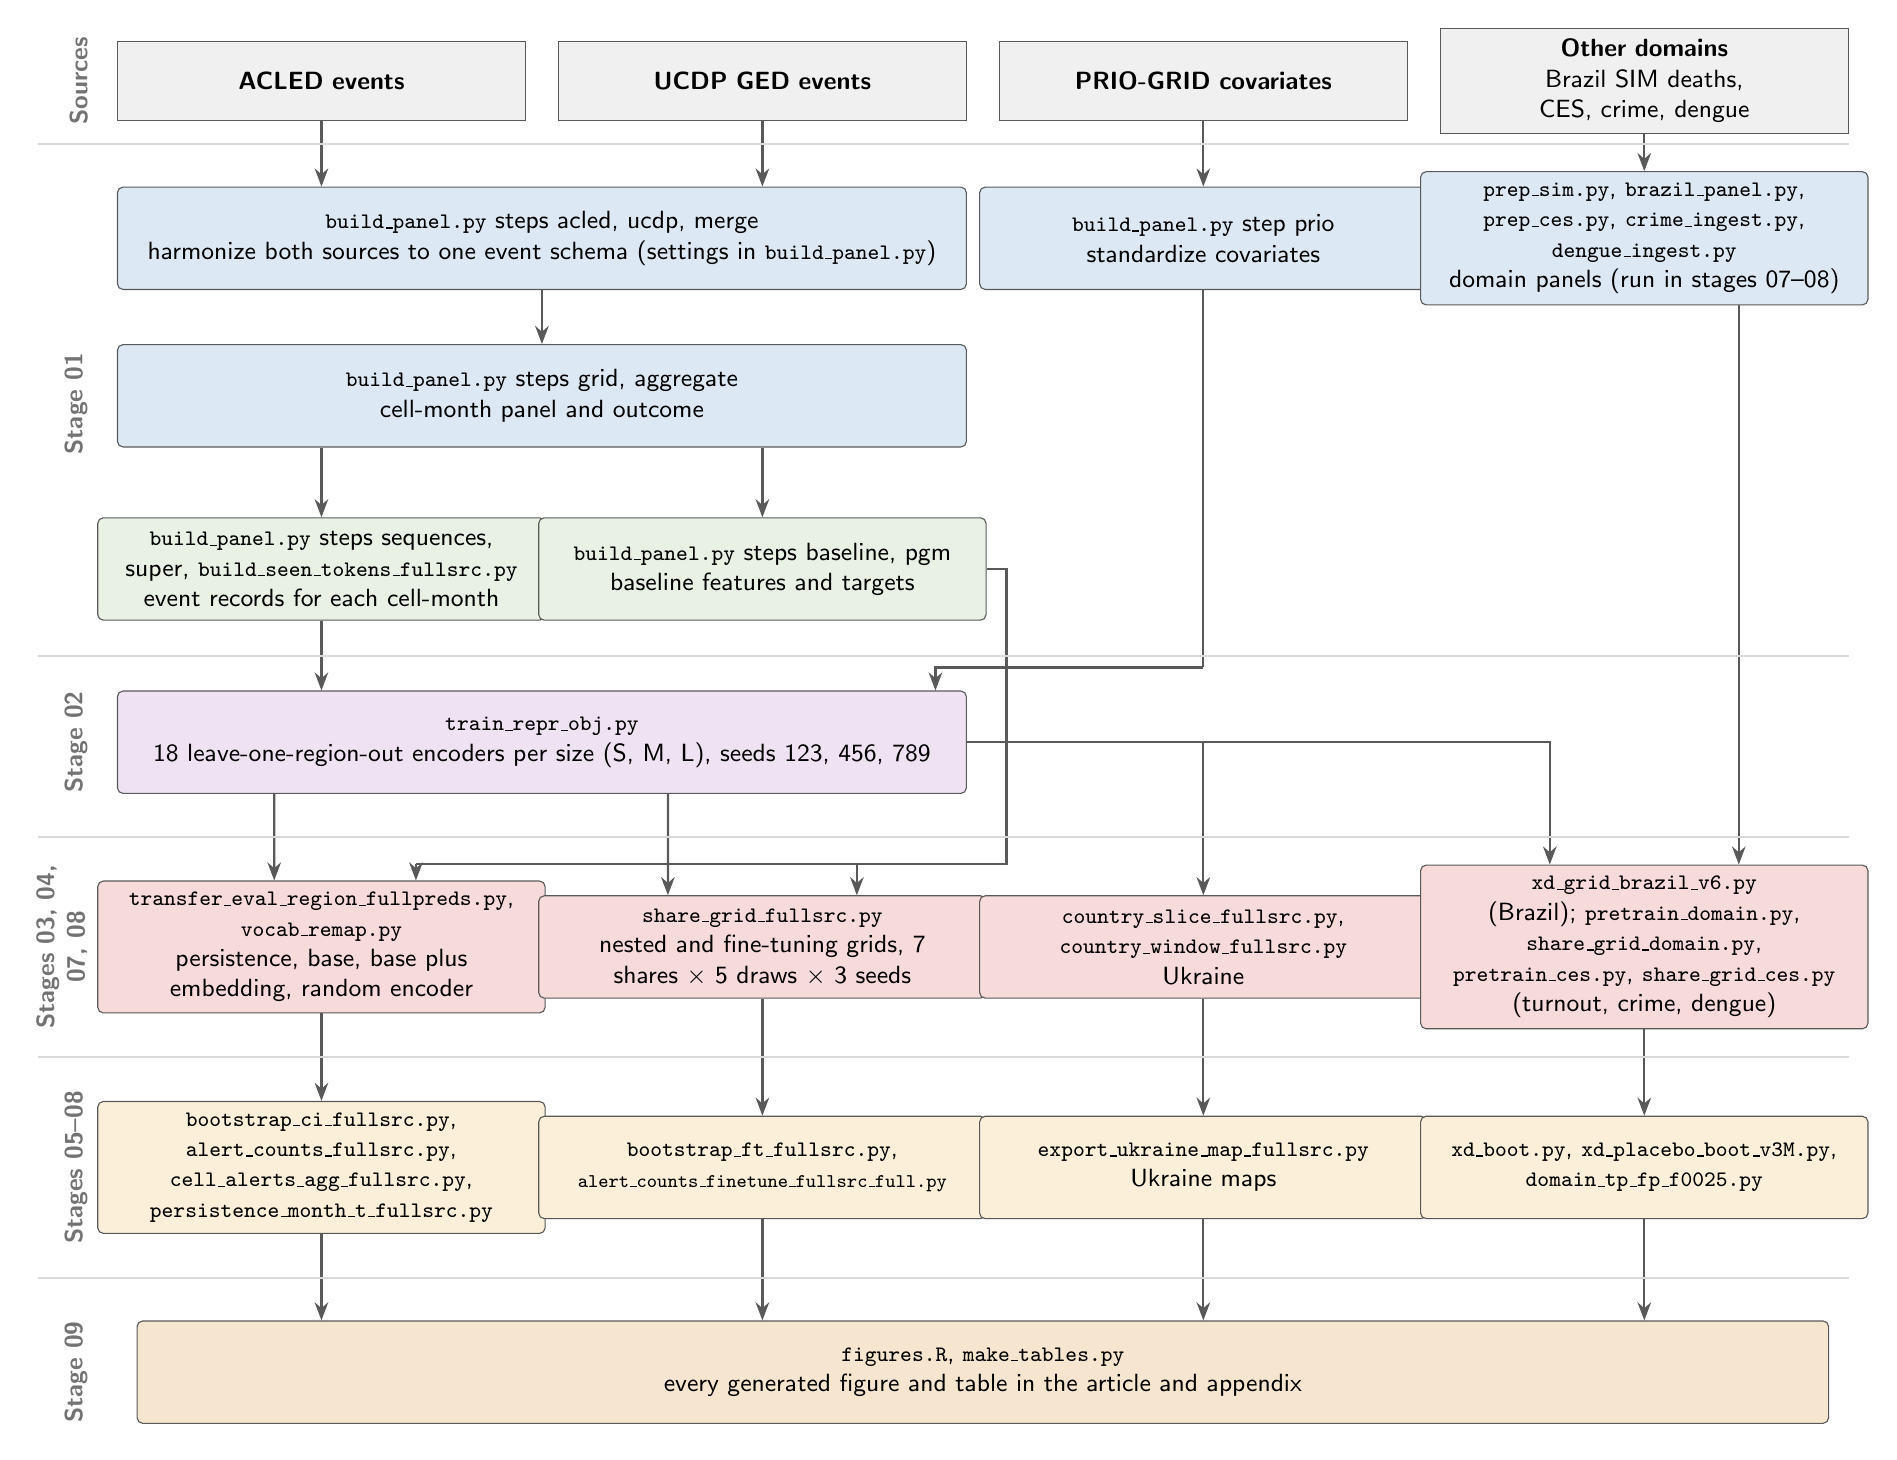
\begin{tikzpicture}[
font=\sffamily\small,
>={Stealth[length=2.3mm]},
sc/.style={draw=black!65, rounded corners=2pt, fill=#1, align=center, inner sep=4pt,
text width=5.4cm, minimum height=1.3cm,
execute at begin node={\hyphenpenalty=10000\exhyphenpenalty=10000}},
sc/.default=white,
src/.style={draw=black!65, fill=black!6, align=center, inner sep=4pt, text width=4.9cm, minimum height=1.0cm},
lane/.style={font=\sffamily\bfseries\small, text=black!55, rotate=90, anchor=south, align=center},
arr/.style={->, thick, draw=black!65},
ln/.style={draw=black!15, thick}
]
\definecolor{cB}{HTML}{DCE9F5}
\definecolor{cF}{HTML}{E8F1E4}
\definecolor{cP}{HTML}{EFE3F3}
\definecolor{cE}{HTML}{F7DADA}
\definecolor{cU}{HTML}{FBEFD9}
\definecolor{cO}{HTML}{F6E6CF}
\providecommand{\scr}[1]{{\ttfamily\footnotesize\bfseries #1}}
\def\xa{0}\def\xb{5.6}\def\xc{11.2}\def\xd{16.8}\def\xab{2.8}

% Sources
\node[src] (acled) at (\xa,0) {\textbf{ACLED events}};
\node[src] (ucdp) at (\xb,0) {\textbf{UCDP GED events}};
\node[src] (prio) at (\xc,0) {\textbf{PRIO-GRID covariates}};
\node[src] (oth) at (\xd,0) {\textbf{Other domains}\\ Brazil SIM deaths, CES, crime, dengue};

% Stage 01: panel and inputs
\node[sc=cB, text width=10.5cm] (ing) at (\xab,-2.0)
{\scr{build\_panel.py} steps acled, ucdp, merge\\
harmonize both sources to one event schema (settings in \scr{build\_panel.py})};
\node[sc=cB] (pst) at (\xc,-2.0) {\scr{build\_panel.py} step prio\\ standardize covariates};
\node[sc=cB] (dom) at (\xd,-2.0) {\scr{prep\_sim.py}, \scr{brazil\_panel.py}, \scr{prep\_ces.py}, \scr{crime\_ingest.py}, \scr{dengue\_ingest.py}\\ domain panels (run in stages 07--08)};
\node[sc=cB, text width=10.5cm] (grd) at (\xab,-4.0)
{\scr{build\_panel.py} steps grid, aggregate\\ cell-month panel and outcome};
\node[sc=cF] (seq) at (\xa,-6.2) {\scr{build\_panel.py} steps sequences, super, \scr{build\_seen\_tokens\_fullsrc.py}\\ event records for each cell-month};
\node[sc=cF] (fea) at (\xb,-6.2) {\scr{build\_panel.py} steps baseline, pgm\\ baseline features and targets};
\draw[arr] (acled) -- (acled |- ing.north);
\draw[arr] (ucdp) -- (ucdp |- ing.north);
\draw[arr] (prio) -- (pst);
\draw[arr] (oth) -- (dom);
\draw[arr] (ing) -- (grd);
\draw[arr] (grd.south -| seq.north) -- (seq.north);
\draw[arr] (grd.south -| fea.north) -- (fea.north);

% Stage 02: pretraining
\node[sc=cP, text width=10.5cm] (pre) at (\xab,-8.4)
{\scr{train\_repr\_obj.py}\\ 18 leave-one-region-out encoders per size (S, M, L), seeds 123, 456, 789};
\draw[arr] (seq) -- (seq |- pre.north);
\draw[thick, draw=black!65] (pst.south) -- (\xc,-7.45);
\draw[arr] (\xc,-7.45) -| ($(pre.north east)+(-0.4,0)$);

% Stages 03, 04, 07, 08: evaluation
\node[sc=cE] (e1) at (\xa,-11.0) {\scr{transfer\_eval\_region\_fullpreds.py}, \scr{vocab\_remap.py}\\ persistence, base, base plus embedding, random encoder};
\node[sc=cE] (e2) at (\xb,-11.0) {\scr{share\_grid\_fullsrc.py}\\ nested and fine-tuning grids, 7 shares $\times$ 5 draws $\times$ 3 seeds};
\node[sc=cE] (e3) at (\xc,-11.0) {\scr{country\_slice\_fullsrc.py}, \scr{country\_window\_fullsrc.py}\\ Ukraine};
\node[sc=cE] (e4) at (\xd,-11.0) {\scr{xd\_grid\_brazil\_v6.py} (Brazil); \scr{pretrain\_domain.py}, \scr{share\_grid\_domain.py}, \scr{pretrain\_ces.py}, \scr{share\_grid\_ces.py} (turnout, crime, dengue)};
\draw[arr] ($(pre.south)+(-3.4,0)$) -- ($(e1.north)+(-0.6,0)$);
\draw[arr] ($(pre.south)+(1.6,0)$) -- ($(e2.north)+(-1.2,0)$);
\draw[arr] (pre.east) -| (e3.north);
\draw[arr] (\xc,-8.4) -- (15.6,-8.4) -- ($(e4.north)+(-1.2,0)$);
\draw[arr] ($(dom.south)+(1.2,0)$) -- ($(e4.north)+(1.2,0)$);
\draw[thick, draw=black!65] (fea.east) -- (8.7,-6.2) -- (8.7,-9.95) -- (1.2,-9.95);
\draw[arr] (1.2,-9.95) -- (1.2,-9.95 |- e1.north);
\draw[arr] (6.8,-9.95) -- (6.8,-9.95 |- e2.north);

% Stages 05, 06, 07, 08: intervals, alerts, maps
\node[sc=cU] (b1) at (\xa,-13.8) {\scr{bootstrap\_ci\_fullsrc.py}, \scr{alert\_counts\_fullsrc.py}, \scr{cell\_alerts\_agg\_fullsrc.py}, \scr{persistence\_month\_t\_fullsrc.py}};
\node[sc=cU] (b2) at (\xb,-13.8) {\scr{bootstrap\_ft\_fullsrc.py},\\ {\ttfamily\scriptsize\bfseries alert\_counts\_finetune\_fullsrc\_full.py}};
\node[sc=cU] (b3) at (\xc,-13.8) {\scr{export\_ukraine\_map\_fullsrc.py}\\ Ukraine maps};
\node[sc=cU] (b4) at (\xd,-13.8) {\scr{xd\_boot.py}, \scr{xd\_placebo\_boot\_v3M.py}, \scr{domain\_tp\_fp\_f0025.py}};
\draw[arr] (e1) -- (b1); \draw[arr] (e2) -- (b2); \draw[arr] (e3) -- (b3); \draw[arr] (e4) -- (b4);

% Stage 09: outputs
\node[sc=cO, text width=21.2cm] (out) at (8.4,-16.4)
{\scr{figures.R}, \scr{make\_tables.py}\\ every generated figure and table in the article and appendix};
\draw[arr] (b1) -- (b1 |- out.north); \draw[arr] (b2) -- (b2 |- out.north);
\draw[arr] (b3) -- (b3 |- out.north); \draw[arr] (b4) -- (b4 |- out.north);

% Lane labels and guides
\foreach \y/\t in {0/Sources, -4.1/Stage 01, -8.4/Stage 02, -11.0/{Stages 03, 04,\\ 07, 08}, -13.8/{Stages 05--08}, -16.4/Stage 09} {
\node[lane] at (-2.85,\y) {\t};
}
\foreach \y in {-0.8, -7.3, -9.6, -12.4, -15.2} {
\draw[ln] (-3.6,\y) -- (19.4,\y);
}
\end{tikzpicture}%
}
\caption{\textbf{Code pipeline.} The driver \texttt{pipeline/run.sh} checks all inputs (stage 00) and then submits stages 01 to 09 as Slurm jobs through one job script, \texttt{pipeline/tasks.sbatch}. Each box names the scripts that perform a step. Every conflict model trains on months through December 2020, and all reported conflict forecasts are for January 2022 onward.}
\label{fig:pipeline}
\end{figure}

\usetikzlibrary{positioning, arrows.meta, calc}
\begin{figure}[!htbp]
\centering
\resizebox{\textwidth}{!}{%
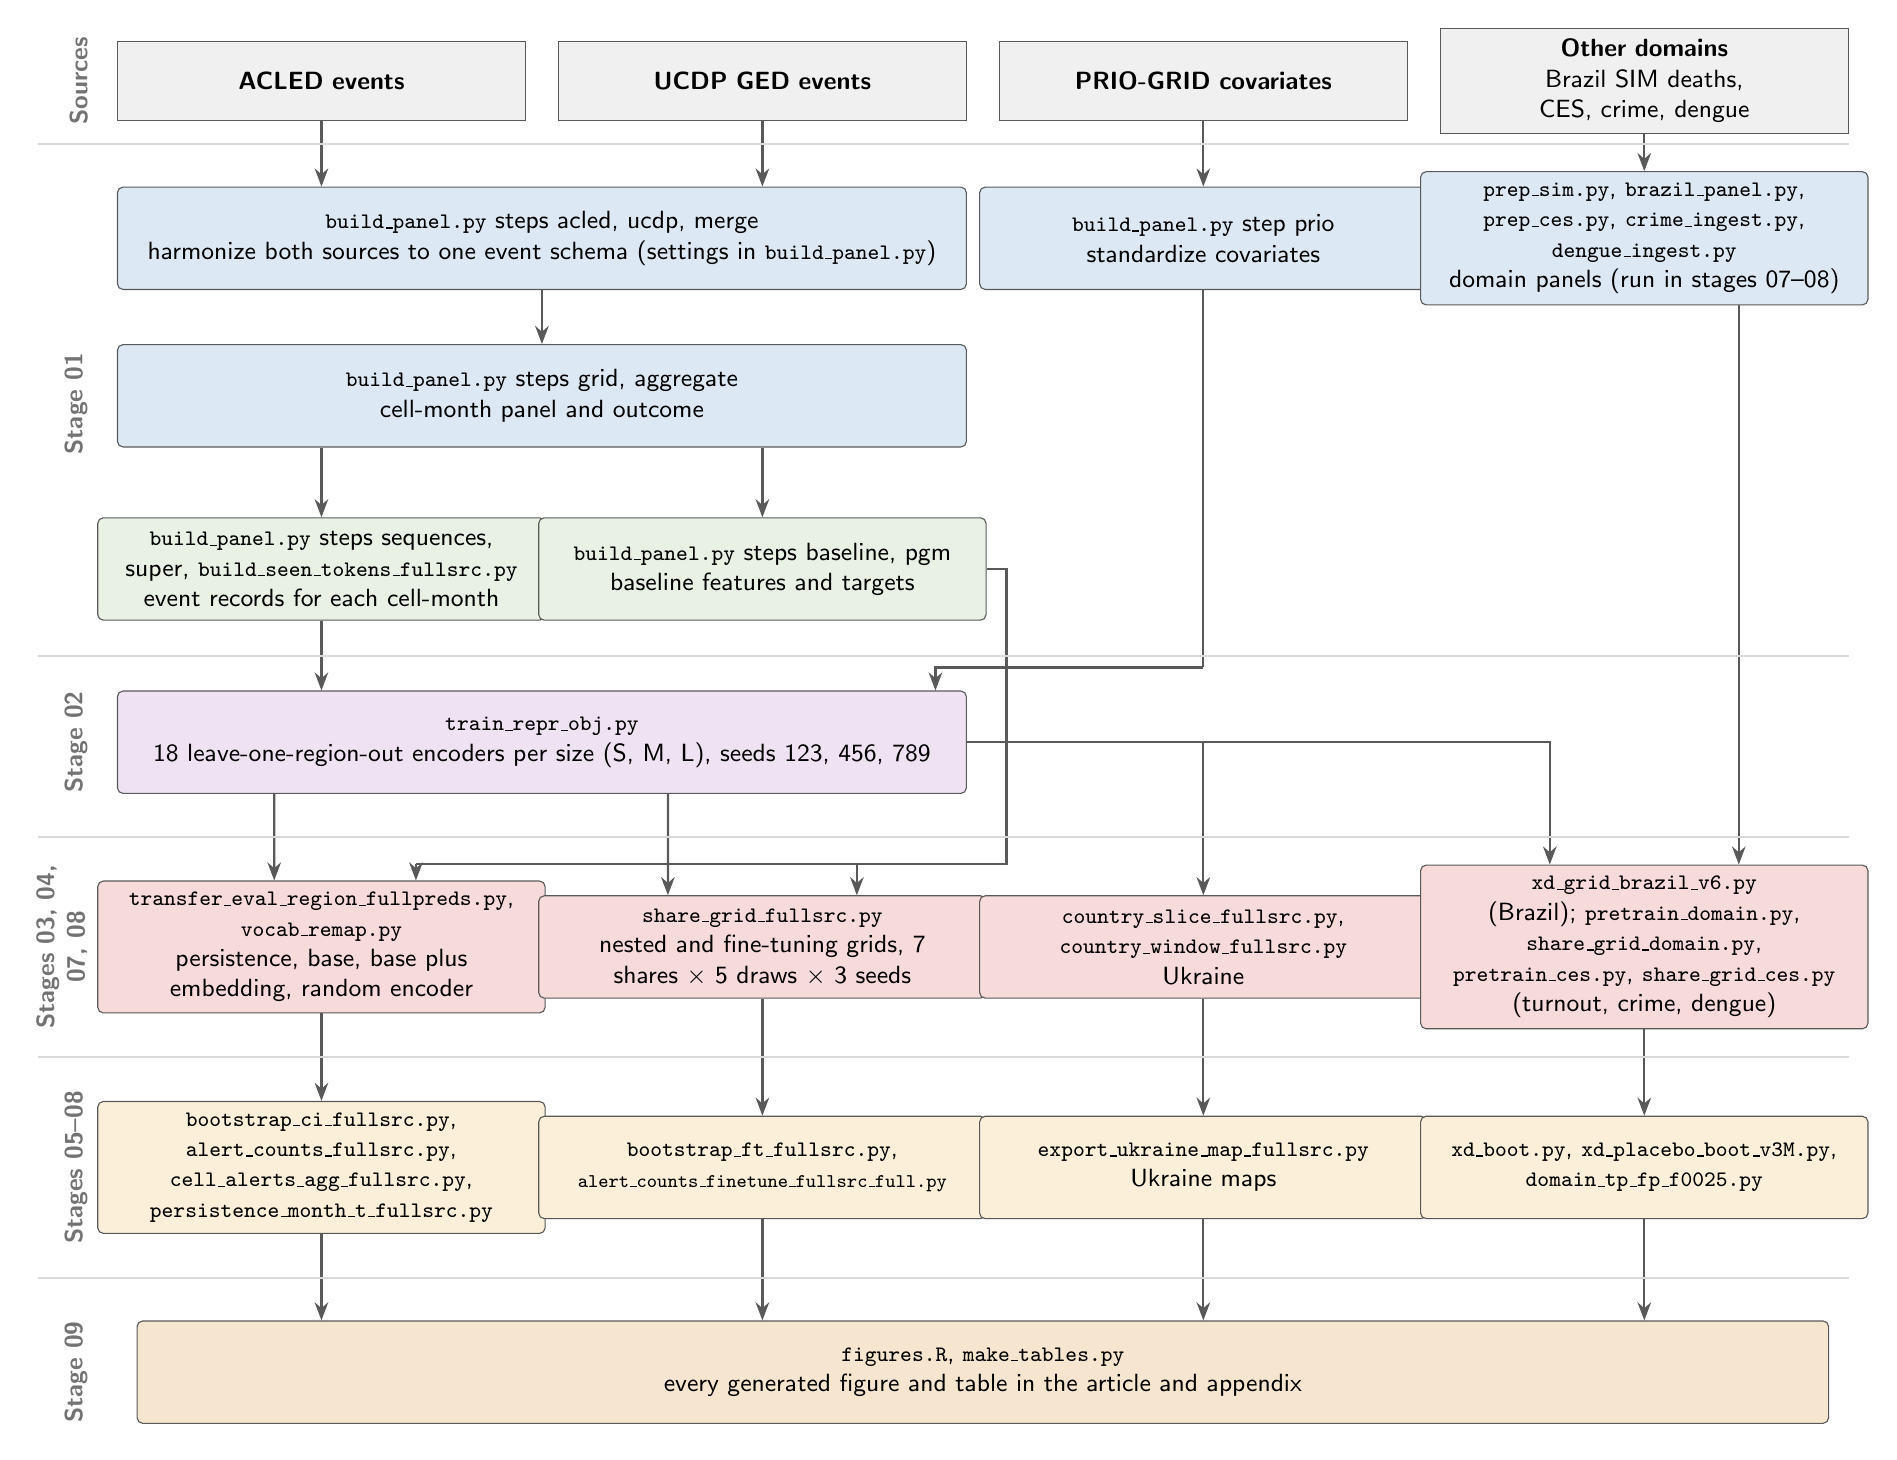
\begin{tikzpicture}[
font=\sffamily\small,
>={Stealth[length=2.3mm]},
sc/.style={draw=black!65, rounded corners=2pt, fill=#1, align=center, inner sep=4pt,
text width=5.4cm, minimum height=1.3cm,
execute at begin node={\hyphenpenalty=10000\exhyphenpenalty=10000}},
sc/.default=white,
src/.style={draw=black!65, fill=black!6, align=center, inner sep=4pt, text width=4.9cm, minimum height=1.0cm},
lane/.style={font=\sffamily\bfseries\small, text=black!55, rotate=90, anchor=south, align=center},
arr/.style={->, thick, draw=black!65},
ln/.style={draw=black!15, thick}
]
\definecolor{cB}{HTML}{DCE9F5}
\definecolor{cF}{HTML}{E8F1E4}
\definecolor{cP}{HTML}{EFE3F3}
\definecolor{cE}{HTML}{F7DADA}
\definecolor{cU}{HTML}{FBEFD9}
\definecolor{cO}{HTML}{F6E6CF}
\providecommand{\scr}[1]{{\ttfamily\footnotesize\bfseries #1}}
\def\xa{0}\def\xb{5.6}\def\xc{11.2}\def\xd{16.8}\def\xab{2.8}

% Sources
\node[src] (acled) at (\xa,0) {\textbf{ACLED events}};
\node[src] (ucdp) at (\xb,0) {\textbf{UCDP GED events}};
\node[src] (prio) at (\xc,0) {\textbf{PRIO-GRID covariates}};
\node[src] (oth) at (\xd,0) {\textbf{Other domains}\\ Brazil SIM deaths, CES, crime, dengue};

% Stage 01: panel and inputs
\node[sc=cB, text width=10.5cm] (ing) at (\xab,-2.0)
{\scr{build\_panel.py} steps acled, ucdp, merge\\
harmonize both sources to one event schema (settings in \scr{build\_panel.py})};
\node[sc=cB] (pst) at (\xc,-2.0) {\scr{build\_panel.py} step prio\\ standardize covariates};
\node[sc=cB] (dom) at (\xd,-2.0) {\scr{prep\_sim.py}, \scr{brazil\_panel.py}, \scr{prep\_ces.py}, \scr{crime\_ingest.py}, \scr{dengue\_ingest.py}\\ domain panels (run in stages 07--08)};
\node[sc=cB, text width=10.5cm] (grd) at (\xab,-4.0)
{\scr{build\_panel.py} steps grid, aggregate\\ cell-month panel and outcome};
\node[sc=cF] (seq) at (\xa,-6.2) {\scr{build\_panel.py} steps sequences, super, \scr{build\_seen\_tokens\_fullsrc.py}\\ event records for each cell-month};
\node[sc=cF] (fea) at (\xb,-6.2) {\scr{build\_panel.py} steps baseline, pgm\\ baseline features and targets};
\draw[arr] (acled) -- (acled |- ing.north);
\draw[arr] (ucdp) -- (ucdp |- ing.north);
\draw[arr] (prio) -- (pst);
\draw[arr] (oth) -- (dom);
\draw[arr] (ing) -- (grd);
\draw[arr] (grd.south -| seq.north) -- (seq.north);
\draw[arr] (grd.south -| fea.north) -- (fea.north);

% Stage 02: pretraining
\node[sc=cP, text width=10.5cm] (pre) at (\xab,-8.4)
{\scr{train\_repr\_obj.py}\\ 18 leave-one-region-out encoders per size (S, M, L), seeds 123, 456, 789};
\draw[arr] (seq) -- (seq |- pre.north);
\draw[thick, draw=black!65] (pst.south) -- (\xc,-7.45);
\draw[arr] (\xc,-7.45) -| ($(pre.north east)+(-0.4,0)$);

% Stages 03, 04, 07, 08: evaluation
\node[sc=cE] (e1) at (\xa,-11.0) {\scr{transfer\_eval\_region\_fullpreds.py}, \scr{vocab\_remap.py}\\ persistence, base, base plus embedding, random encoder};
\node[sc=cE] (e2) at (\xb,-11.0) {\scr{share\_grid\_fullsrc.py}\\ nested and fine-tuning grids, 7 shares $\times$ 5 draws $\times$ 3 seeds};
\node[sc=cE] (e3) at (\xc,-11.0) {\scr{country\_slice\_fullsrc.py}, \scr{country\_window\_fullsrc.py}\\ Ukraine};
\node[sc=cE] (e4) at (\xd,-11.0) {\scr{xd\_grid\_brazil\_v6.py} (Brazil); \scr{pretrain\_domain.py}, \scr{share\_grid\_domain.py}, \scr{pretrain\_ces.py}, \scr{share\_grid\_ces.py} (turnout, crime, dengue)};
\draw[arr] ($(pre.south)+(-3.4,0)$) -- ($(e1.north)+(-0.6,0)$);
\draw[arr] ($(pre.south)+(1.6,0)$) -- ($(e2.north)+(-1.2,0)$);
\draw[arr] (pre.east) -| (e3.north);
\draw[arr] (\xc,-8.4) -- (15.6,-8.4) -- ($(e4.north)+(-1.2,0)$);
\draw[arr] ($(dom.south)+(1.2,0)$) -- ($(e4.north)+(1.2,0)$);
\draw[thick, draw=black!65] (fea.east) -- (8.7,-6.2) -- (8.7,-9.95) -- (1.2,-9.95);
\draw[arr] (1.2,-9.95) -- (1.2,-9.95 |- e1.north);
\draw[arr] (6.8,-9.95) -- (6.8,-9.95 |- e2.north);

% Stages 05, 06, 07, 08: intervals, alerts, maps
\node[sc=cU] (b1) at (\xa,-13.8) {\scr{bootstrap\_ci\_fullsrc.py}, \scr{alert\_counts\_fullsrc.py}, \scr{cell\_alerts\_agg\_fullsrc.py}, \scr{persistence\_month\_t\_fullsrc.py}};
\node[sc=cU] (b2) at (\xb,-13.8) {\scr{bootstrap\_ft\_fullsrc.py},\\ {\ttfamily\scriptsize\bfseries alert\_counts\_finetune\_fullsrc\_full.py}};
\node[sc=cU] (b3) at (\xc,-13.8) {\scr{export\_ukraine\_map\_fullsrc.py}\\ Ukraine maps};
\node[sc=cU] (b4) at (\xd,-13.8) {\scr{xd\_boot.py}, \scr{xd\_placebo\_boot\_v3M.py}, \scr{domain\_tp\_fp\_f0025.py}};
\draw[arr] (e1) -- (b1); \draw[arr] (e2) -- (b2); \draw[arr] (e3) -- (b3); \draw[arr] (e4) -- (b4);

% Stage 09: outputs
\node[sc=cO, text width=21.2cm] (out) at (8.4,-16.4)
{\scr{figures.R}, \scr{make\_tables.py}\\ every generated figure and table in the article and appendix};
\draw[arr] (b1) -- (b1 |- out.north); \draw[arr] (b2) -- (b2 |- out.north);
\draw[arr] (b3) -- (b3 |- out.north); \draw[arr] (b4) -- (b4 |- out.north);

% Lane labels and guides
\foreach \y/\t in {0/Sources, -4.1/Stage 01, -8.4/Stage 02, -11.0/{Stages 03, 04,\\ 07, 08}, -13.8/{Stages 05--08}, -16.4/Stage 09} {
\node[lane] at (-2.85,\y) {\t};
}
\foreach \y in {-0.8, -7.3, -9.6, -12.4, -15.2} {
\draw[ln] (-3.6,\y) -- (19.4,\y);
}
\end{tikzpicture}%
}
\caption{\textbf{Code pipeline.} The driver \texttt{pipeline/run.sh} checks all inputs (stage 00) and then submits stages 01 to 09 as Slurm jobs through one job script, \texttt{pipeline/tasks.sbatch}. Each box names the scripts that perform a step. Every conflict model trains on months through December 2020, and all reported conflict forecasts are for January 2022 onward.}
\label{fig:pipeline}
\end{figure}

\usetikzlibrary{positioning, arrows.meta, calc}
\begin{figure}[!htbp]
\centering
\resizebox{\textwidth}{!}{%
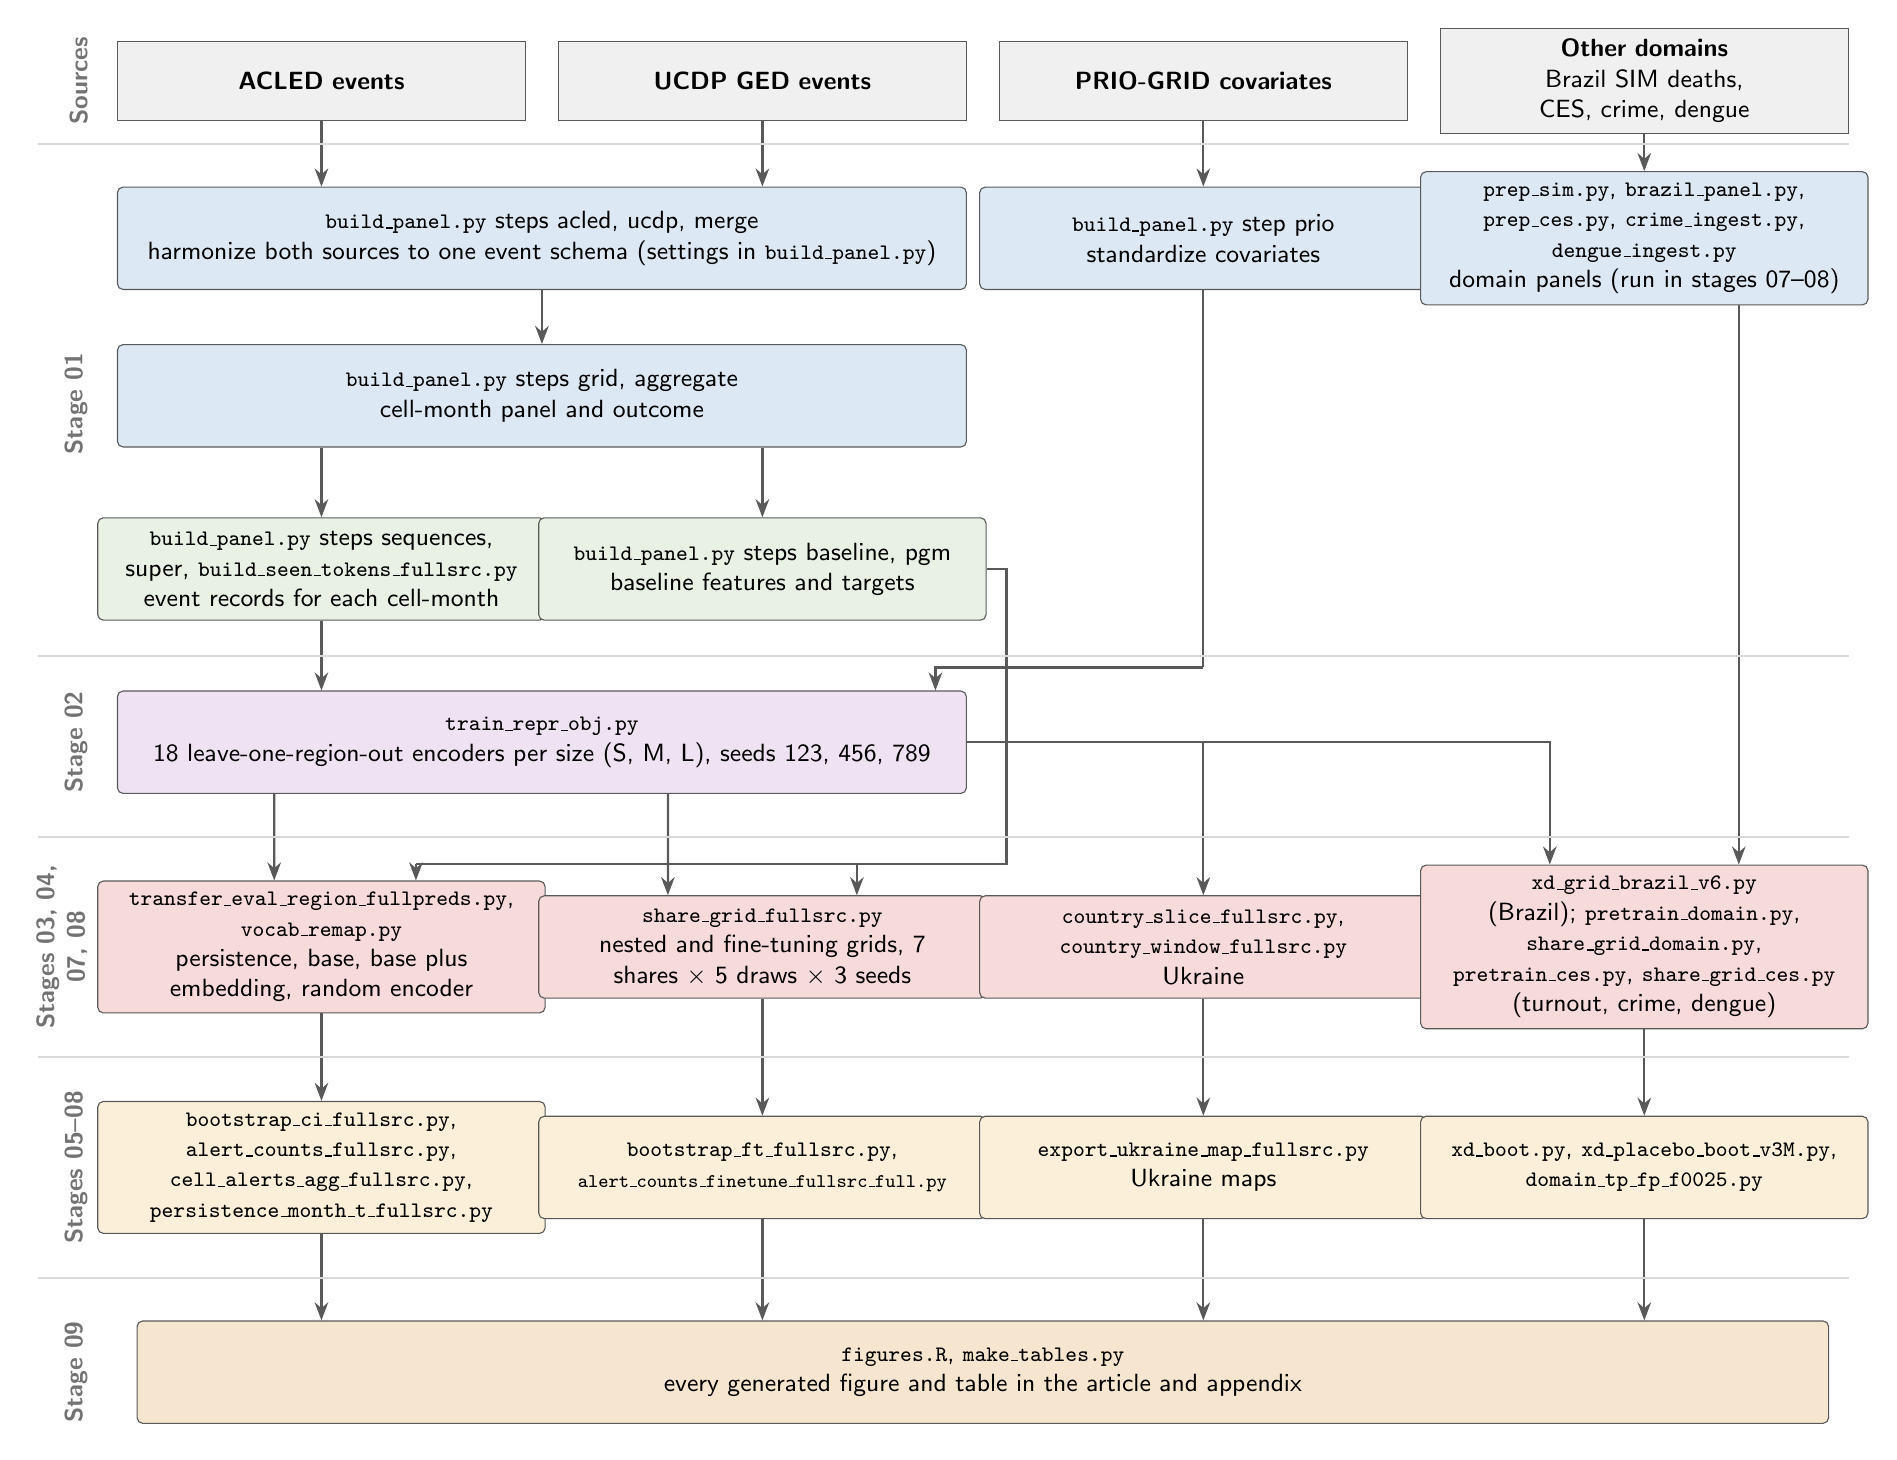
\begin{tikzpicture}[
font=\sffamily\small,
>={Stealth[length=2.3mm]},
sc/.style={draw=black!65, rounded corners=2pt, fill=#1, align=center, inner sep=4pt,
text width=5.4cm, minimum height=1.3cm,
execute at begin node={\hyphenpenalty=10000\exhyphenpenalty=10000}},
sc/.default=white,
src/.style={draw=black!65, fill=black!6, align=center, inner sep=4pt, text width=4.9cm, minimum height=1.0cm},
lane/.style={font=\sffamily\bfseries\small, text=black!55, rotate=90, anchor=south, align=center},
arr/.style={->, thick, draw=black!65},
ln/.style={draw=black!15, thick}
]
\definecolor{cB}{HTML}{DCE9F5}
\definecolor{cF}{HTML}{E8F1E4}
\definecolor{cP}{HTML}{EFE3F3}
\definecolor{cE}{HTML}{F7DADA}
\definecolor{cU}{HTML}{FBEFD9}
\definecolor{cO}{HTML}{F6E6CF}
\providecommand{\scr}[1]{{\ttfamily\footnotesize\bfseries #1}}
\def\xa{0}\def\xb{5.6}\def\xc{11.2}\def\xd{16.8}\def\xab{2.8}

% Sources
\node[src] (acled) at (\xa,0) {\textbf{ACLED events}};
\node[src] (ucdp) at (\xb,0) {\textbf{UCDP GED events}};
\node[src] (prio) at (\xc,0) {\textbf{PRIO-GRID covariates}};
\node[src] (oth) at (\xd,0) {\textbf{Other domains}\\ Brazil SIM deaths, CES, crime, dengue};

% Stage 01: panel and inputs
\node[sc=cB, text width=10.5cm] (ing) at (\xab,-2.0)
{\scr{build\_panel.py} steps acled, ucdp, merge\\
harmonize both sources to one event schema (settings in \scr{build\_panel.py})};
\node[sc=cB] (pst) at (\xc,-2.0) {\scr{build\_panel.py} step prio\\ standardize covariates};
\node[sc=cB] (dom) at (\xd,-2.0) {\scr{prep\_sim.py}, \scr{brazil\_panel.py}, \scr{prep\_ces.py}, \scr{crime\_ingest.py}, \scr{dengue\_ingest.py}\\ domain panels (run in stages 07--08)};
\node[sc=cB, text width=10.5cm] (grd) at (\xab,-4.0)
{\scr{build\_panel.py} steps grid, aggregate\\ cell-month panel and outcome};
\node[sc=cF] (seq) at (\xa,-6.2) {\scr{build\_panel.py} steps sequences, super, \scr{build\_seen\_tokens\_fullsrc.py}\\ event records for each cell-month};
\node[sc=cF] (fea) at (\xb,-6.2) {\scr{build\_panel.py} steps baseline, pgm\\ baseline features and targets};
\draw[arr] (acled) -- (acled |- ing.north);
\draw[arr] (ucdp) -- (ucdp |- ing.north);
\draw[arr] (prio) -- (pst);
\draw[arr] (oth) -- (dom);
\draw[arr] (ing) -- (grd);
\draw[arr] (grd.south -| seq.north) -- (seq.north);
\draw[arr] (grd.south -| fea.north) -- (fea.north);

% Stage 02: pretraining
\node[sc=cP, text width=10.5cm] (pre) at (\xab,-8.4)
{\scr{train\_repr\_obj.py}\\ 18 leave-one-region-out encoders per size (S, M, L), seeds 123, 456, 789};
\draw[arr] (seq) -- (seq |- pre.north);
\draw[thick, draw=black!65] (pst.south) -- (\xc,-7.45);
\draw[arr] (\xc,-7.45) -| ($(pre.north east)+(-0.4,0)$);

% Stages 03, 04, 07, 08: evaluation
\node[sc=cE] (e1) at (\xa,-11.0) {\scr{transfer\_eval\_region\_fullpreds.py}, \scr{vocab\_remap.py}\\ persistence, base, base plus embedding, random encoder};
\node[sc=cE] (e2) at (\xb,-11.0) {\scr{share\_grid\_fullsrc.py}\\ nested and fine-tuning grids, 7 shares $\times$ 5 draws $\times$ 3 seeds};
\node[sc=cE] (e3) at (\xc,-11.0) {\scr{country\_slice\_fullsrc.py}, \scr{country\_window\_fullsrc.py}\\ Ukraine};
\node[sc=cE] (e4) at (\xd,-11.0) {\scr{xd\_grid\_brazil\_v6.py} (Brazil); \scr{pretrain\_domain.py}, \scr{share\_grid\_domain.py}, \scr{pretrain\_ces.py}, \scr{share\_grid\_ces.py} (turnout, crime, dengue)};
\draw[arr] ($(pre.south)+(-3.4,0)$) -- ($(e1.north)+(-0.6,0)$);
\draw[arr] ($(pre.south)+(1.6,0)$) -- ($(e2.north)+(-1.2,0)$);
\draw[arr] (pre.east) -| (e3.north);
\draw[arr] (\xc,-8.4) -- (15.6,-8.4) -- ($(e4.north)+(-1.2,0)$);
\draw[arr] ($(dom.south)+(1.2,0)$) -- ($(e4.north)+(1.2,0)$);
\draw[thick, draw=black!65] (fea.east) -- (8.7,-6.2) -- (8.7,-9.95) -- (1.2,-9.95);
\draw[arr] (1.2,-9.95) -- (1.2,-9.95 |- e1.north);
\draw[arr] (6.8,-9.95) -- (6.8,-9.95 |- e2.north);

% Stages 05, 06, 07, 08: intervals, alerts, maps
\node[sc=cU] (b1) at (\xa,-13.8) {\scr{bootstrap\_ci\_fullsrc.py}, \scr{alert\_counts\_fullsrc.py}, \scr{cell\_alerts\_agg\_fullsrc.py}, \scr{persistence\_month\_t\_fullsrc.py}};
\node[sc=cU] (b2) at (\xb,-13.8) {\scr{bootstrap\_ft\_fullsrc.py},\\ {\ttfamily\scriptsize\bfseries alert\_counts\_finetune\_fullsrc\_full.py}};
\node[sc=cU] (b3) at (\xc,-13.8) {\scr{export\_ukraine\_map\_fullsrc.py}\\ Ukraine maps};
\node[sc=cU] (b4) at (\xd,-13.8) {\scr{xd\_boot.py}, \scr{xd\_placebo\_boot\_v3M.py}, \scr{domain\_tp\_fp\_f0025.py}};
\draw[arr] (e1) -- (b1); \draw[arr] (e2) -- (b2); \draw[arr] (e3) -- (b3); \draw[arr] (e4) -- (b4);

% Stage 09: outputs
\node[sc=cO, text width=21.2cm] (out) at (8.4,-16.4)
{\scr{figures.R}, \scr{make\_tables.py}\\ every generated figure and table in the article and appendix};
\draw[arr] (b1) -- (b1 |- out.north); \draw[arr] (b2) -- (b2 |- out.north);
\draw[arr] (b3) -- (b3 |- out.north); \draw[arr] (b4) -- (b4 |- out.north);

% Lane labels and guides
\foreach \y/\t in {0/Sources, -4.1/Stage 01, -8.4/Stage 02, -11.0/{Stages 03, 04,\\ 07, 08}, -13.8/{Stages 05--08}, -16.4/Stage 09} {
\node[lane] at (-2.85,\y) {\t};
}
\foreach \y in {-0.8, -7.3, -9.6, -12.4, -15.2} {
\draw[ln] (-3.6,\y) -- (19.4,\y);
}
\end{tikzpicture}%
}
\caption{\textbf{Code pipeline.} The driver \texttt{pipeline/run.sh} checks all inputs (stage 00) and then submits stages 01 to 09 as Slurm jobs through one job script, \texttt{pipeline/tasks.sbatch}. Each box names the scripts that perform a step. Every conflict model trains on months through December 2020, and all reported conflict forecasts are for January 2022 onward.}
\label{fig:pipeline}
\end{figure}

\usetikzlibrary{positioning, arrows.meta, calc}
\begin{figure}[!htbp]
\centering
\resizebox{\textwidth}{!}{%
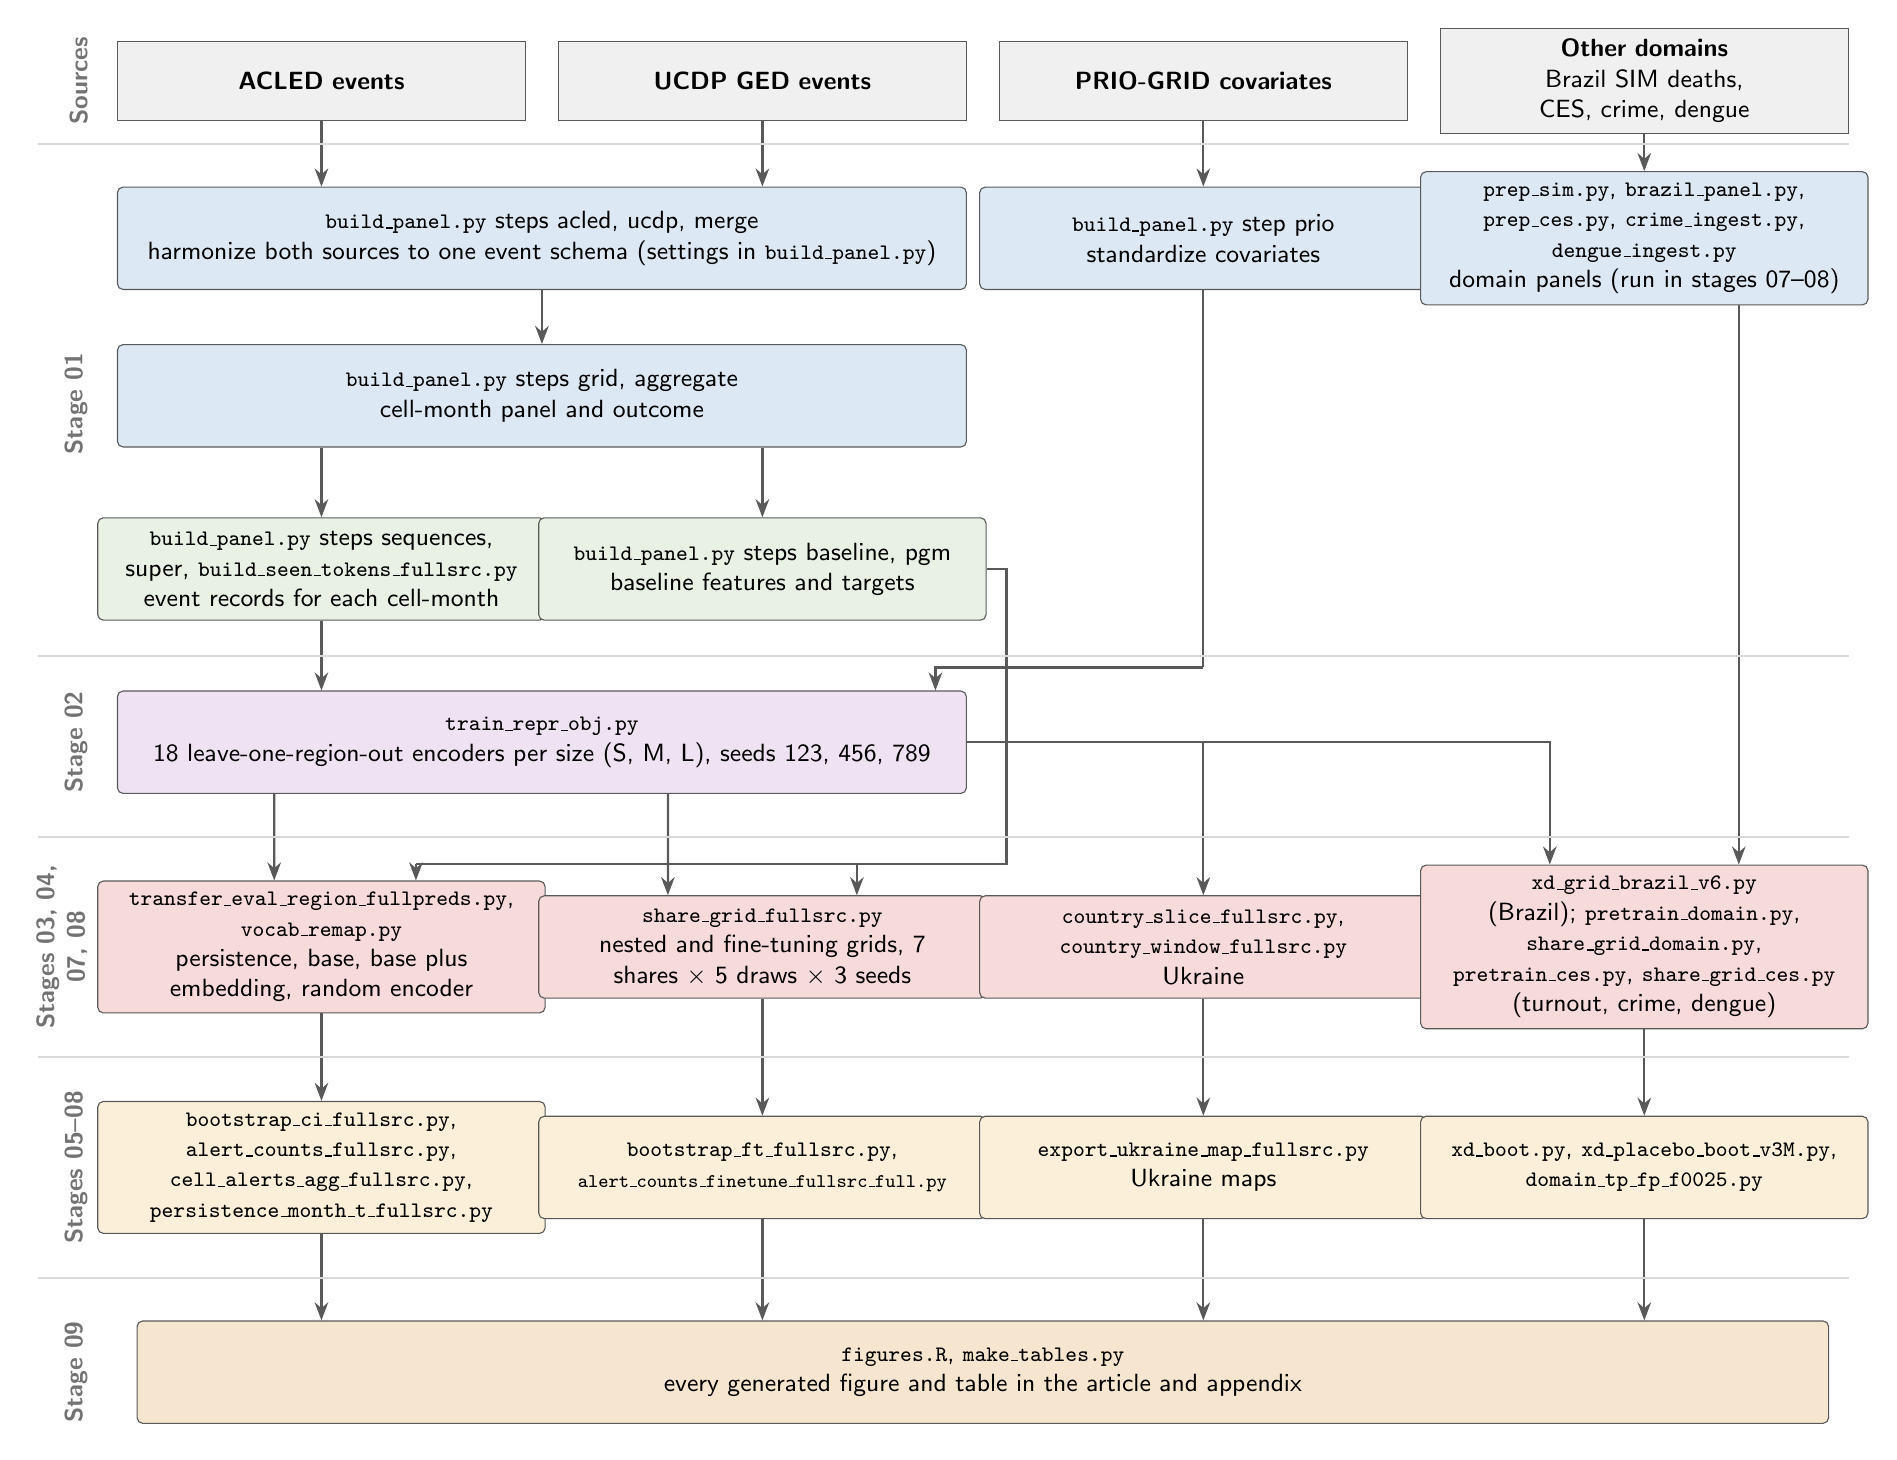
\begin{tikzpicture}[
font=\sffamily\small,
>={Stealth[length=2.3mm]},
sc/.style={draw=black!65, rounded corners=2pt, fill=#1, align=center, inner sep=4pt,
text width=5.4cm, minimum height=1.3cm,
execute at begin node={\hyphenpenalty=10000\exhyphenpenalty=10000}},
sc/.default=white,
src/.style={draw=black!65, fill=black!6, align=center, inner sep=4pt, text width=4.9cm, minimum height=1.0cm},
lane/.style={font=\sffamily\bfseries\small, text=black!55, rotate=90, anchor=south, align=center},
arr/.style={->, thick, draw=black!65},
ln/.style={draw=black!15, thick}
]
\definecolor{cB}{HTML}{DCE9F5}
\definecolor{cF}{HTML}{E8F1E4}
\definecolor{cP}{HTML}{EFE3F3}
\definecolor{cE}{HTML}{F7DADA}
\definecolor{cU}{HTML}{FBEFD9}
\definecolor{cO}{HTML}{F6E6CF}
\providecommand{\scr}[1]{{\ttfamily\footnotesize\bfseries #1}}
\def\xa{0}\def\xb{5.6}\def\xc{11.2}\def\xd{16.8}\def\xab{2.8}

% Sources
\node[src] (acled) at (\xa,0) {\textbf{ACLED events}};
\node[src] (ucdp) at (\xb,0) {\textbf{UCDP GED events}};
\node[src] (prio) at (\xc,0) {\textbf{PRIO-GRID covariates}};
\node[src] (oth) at (\xd,0) {\textbf{Other domains}\\ Brazil SIM deaths, CES, crime, dengue};

% Stage 01: panel and inputs
\node[sc=cB, text width=10.5cm] (ing) at (\xab,-2.0)
{\scr{build\_panel.py} steps acled, ucdp, merge\\
harmonize both sources to one event schema (settings in \scr{build\_panel.py})};
\node[sc=cB] (pst) at (\xc,-2.0) {\scr{build\_panel.py} step prio\\ standardize covariates};
\node[sc=cB] (dom) at (\xd,-2.0) {\scr{prep\_sim.py}, \scr{brazil\_panel.py}, \scr{prep\_ces.py}, \scr{crime\_ingest.py}, \scr{dengue\_ingest.py}\\ domain panels (run in stages 07--08)};
\node[sc=cB, text width=10.5cm] (grd) at (\xab,-4.0)
{\scr{build\_panel.py} steps grid, aggregate\\ cell-month panel and outcome};
\node[sc=cF] (seq) at (\xa,-6.2) {\scr{build\_panel.py} steps sequences, super, \scr{build\_seen\_tokens\_fullsrc.py}\\ event records for each cell-month};
\node[sc=cF] (fea) at (\xb,-6.2) {\scr{build\_panel.py} steps baseline, pgm\\ baseline features and targets};
\draw[arr] (acled) -- (acled |- ing.north);
\draw[arr] (ucdp) -- (ucdp |- ing.north);
\draw[arr] (prio) -- (pst);
\draw[arr] (oth) -- (dom);
\draw[arr] (ing) -- (grd);
\draw[arr] (grd.south -| seq.north) -- (seq.north);
\draw[arr] (grd.south -| fea.north) -- (fea.north);

% Stage 02: pretraining
\node[sc=cP, text width=10.5cm] (pre) at (\xab,-8.4)
{\scr{train\_repr\_obj.py}\\ 18 leave-one-region-out encoders per size (S, M, L), seeds 123, 456, 789};
\draw[arr] (seq) -- (seq |- pre.north);
\draw[thick, draw=black!65] (pst.south) -- (\xc,-7.45);
\draw[arr] (\xc,-7.45) -| ($(pre.north east)+(-0.4,0)$);

% Stages 03, 04, 07, 08: evaluation
\node[sc=cE] (e1) at (\xa,-11.0) {\scr{transfer\_eval\_region\_fullpreds.py}, \scr{vocab\_remap.py}\\ persistence, base, base plus embedding, random encoder};
\node[sc=cE] (e2) at (\xb,-11.0) {\scr{share\_grid\_fullsrc.py}\\ nested and fine-tuning grids, 7 shares $\times$ 5 draws $\times$ 3 seeds};
\node[sc=cE] (e3) at (\xc,-11.0) {\scr{country\_slice\_fullsrc.py}, \scr{country\_window\_fullsrc.py}\\ Ukraine};
\node[sc=cE] (e4) at (\xd,-11.0) {\scr{xd\_grid\_brazil\_v6.py} (Brazil); \scr{pretrain\_domain.py}, \scr{share\_grid\_domain.py}, \scr{pretrain\_ces.py}, \scr{share\_grid\_ces.py} (turnout, crime, dengue)};
\draw[arr] ($(pre.south)+(-3.4,0)$) -- ($(e1.north)+(-0.6,0)$);
\draw[arr] ($(pre.south)+(1.6,0)$) -- ($(e2.north)+(-1.2,0)$);
\draw[arr] (pre.east) -| (e3.north);
\draw[arr] (\xc,-8.4) -- (15.6,-8.4) -- ($(e4.north)+(-1.2,0)$);
\draw[arr] ($(dom.south)+(1.2,0)$) -- ($(e4.north)+(1.2,0)$);
\draw[thick, draw=black!65] (fea.east) -- (8.7,-6.2) -- (8.7,-9.95) -- (1.2,-9.95);
\draw[arr] (1.2,-9.95) -- (1.2,-9.95 |- e1.north);
\draw[arr] (6.8,-9.95) -- (6.8,-9.95 |- e2.north);

% Stages 05, 06, 07, 08: intervals, alerts, maps
\node[sc=cU] (b1) at (\xa,-13.8) {\scr{bootstrap\_ci\_fullsrc.py}, \scr{alert\_counts\_fullsrc.py}, \scr{cell\_alerts\_agg\_fullsrc.py}, \scr{persistence\_month\_t\_fullsrc.py}};
\node[sc=cU] (b2) at (\xb,-13.8) {\scr{bootstrap\_ft\_fullsrc.py},\\ {\ttfamily\scriptsize\bfseries alert\_counts\_finetune\_fullsrc\_full.py}};
\node[sc=cU] (b3) at (\xc,-13.8) {\scr{export\_ukraine\_map\_fullsrc.py}\\ Ukraine maps};
\node[sc=cU] (b4) at (\xd,-13.8) {\scr{xd\_boot.py}, \scr{xd\_placebo\_boot\_v3M.py}, \scr{domain\_tp\_fp\_f0025.py}};
\draw[arr] (e1) -- (b1); \draw[arr] (e2) -- (b2); \draw[arr] (e3) -- (b3); \draw[arr] (e4) -- (b4);

% Stage 09: outputs
\node[sc=cO, text width=21.2cm] (out) at (8.4,-16.4)
{\scr{figures.R}, \scr{make\_tables.py}\\ every generated figure and table in the article and appendix};
\draw[arr] (b1) -- (b1 |- out.north); \draw[arr] (b2) -- (b2 |- out.north);
\draw[arr] (b3) -- (b3 |- out.north); \draw[arr] (b4) -- (b4 |- out.north);

% Lane labels and guides
\foreach \y/\t in {0/Sources, -4.1/Stage 01, -8.4/Stage 02, -11.0/{Stages 03, 04,\\ 07, 08}, -13.8/{Stages 05--08}, -16.4/Stage 09} {
\node[lane] at (-2.85,\y) {\t};
}
\foreach \y in {-0.8, -7.3, -9.6, -12.4, -15.2} {
\draw[ln] (-3.6,\y) -- (19.4,\y);
}
\end{tikzpicture}%
}
\caption{\textbf{Code pipeline.} The driver \texttt{pipeline/run.sh} checks all inputs (stage 00) and then submits stages 01 to 09 as Slurm jobs through one job script, \texttt{pipeline/tasks.sbatch}. Each box names the scripts that perform a step. Every conflict model trains on months through December 2020, and all reported conflict forecasts are for January 2022 onward.}
\label{fig:pipeline}
\end{figure}
